\makeatletter
\@ifundefined{bwtrue}{\newif\ifbw\bwfalse}{}
\@ifundefined{acmtrue}{\newif\ifacm\acmtrue}{}
\makeatother
\makeatletter
\let\@period=\,
\makeatother
\documentclass[a4paper]{article}
\usepackage{xspace}
\usepackage{color}
\usepackage[leqno]{amsmath}
\usepackage{amssymb}
\usepackage{array}
\usepackage{tabularx}
\usepackage{booktabs}
\usepackage{url}
\usepackage{hyperref}
\usepackage{breakurl}
\usepackage{graphicx}
\usepackage{subfigure}
\usepackage{epsfig}
\usepackage[draft]{fixme}
\newif\ifcomments
\commentsfalse
\usepackage{url}
\makeatletter
\def\url@leostyle{%
  \@ifundefined{selectfont}{\def\UrlFont{\small\sf}}{\def\UrlFont{\small\sf}}}
\makeatother
\urlstyle{leo}
\usepackage[normalem]{ulem}
\usepackage{xspace}
%same notation policy for each instance of figure, thm, etc
\newcommand{\myfig}{Fig.~}
\newcommand{\mytab}{Tab.~}
\newcommand{\mysec}{Sec.~}
\newcommand{\mychap}{Chap.~}
\newcommand{\myapp}{App.~}
\newcommand{\etal}{et~al.\xspace}
\newcommand{\wrt}{w.r.t.\xspace}
\newcommand{\eg}{e.g.\xspace}
\newcommand{\ie}{i.e.\xspace}
\newcommand{\etc}{etc.\xspace}
\newcommand{\cf}{see\xspace}

%les maths comme au lycee
\let\eset\emptyset
\newcommand{\rplus}[1]{\mathop{{#1}^{+}}}
\newcommand{\rstar}[1]{\mathop{{#1}^{*}}}
\newcommand{\transc}[1]{\mathop{{#1}^{+}}}
\newcommand{\maybe}[1]{\mathop{{#1}^{?}}}

%def
  \newcommand{\dfnshort}[2]{{#1}\triangleq{#2}}
  \newcommand{\dfn}[2]{{#1}~\triangleq~{#2}}

%sets
\newcommand{\setcal}[1]{\mathcal{#1} }
\newcommand{\setbf}[1]{\mathbb{#1} }
\newcommand{\setfrak}[1]{\mathfrak{#1} }


  %writes, reads, barriers
  \let\setset\setbf
  \newcommand{\evts}{\setset{E}}

  \newcommand{\lwf}{\textsf{fence}}
  \newcommand{\mfence}{\ensuremath{\mathsf{mfence}}}
  \newcommand{\lwfence}{\ensuremath{\mathsf{fence}}}
  \newcommand{\ff}{\textsf{fence.sc}}
  \newcommand{\ffence}{\ensuremath{\mathsf{f{\kern-0.1em}fence}}}
  \newcommand{\fences}{\ensuremath{\mathsf{fence}}}
  \newcommand{\relw}{\ensuremath{\mathsf{rel}}}
  \newcommand{\acqr}{\ensuremath{\mathsf{acq}}}
  \newcommand{\cumul}{\ensuremath{\mathsf{cumul}}}
  \newcommand{\Acumul}{\ensuremath{\mathsf{A{\kern-0.3em}-{\kern-0.3em}cumul}}}

  %procs
  \newcommand{\pr}{\operatorname{proc}}

  %locs
  \newcommand{\lo}{\ell}
  \newcommand{\loc}{\operatorname{addr}}

  %vals 
  \newcommand{\val}{\operatorname{val}}

%relations
\newcommand{\stacklabel}[1]
%{\stackrel{\smash{\scriptscriptstyle\#1}}}
{\stackrel{\smash{\scriptstyle\textnormal{#1}}}}
  %any
  \newcommand{\rln}[1]{\ensuremath{\xrightarrow{#1}}}

  %po
  \newcommand{\iico}{\ensuremath{\mathsf{ii}}}
  \newcommand{\ctrlcfence}{\ensuremath{\mathsf{ctrlcfence}}}
  \newcommand{\ctrl}{\ensuremath{\mathsf{ctrl}}}
  \newcommand{\data}{\ensuremath{\mathsf{data}}}
  \newcommand{\addr}{\ensuremath{\mathsf{addr}}}
  \newcommand{\ddreg}{\ensuremath{\mathsf{dd}}}
  \newcommand{\rfreg}{{\mathsf{rfreg}}}
  \newcommand{\isb}{\ensuremath{\mathsf{isb}}}
  \newcommand{\isync}{\ensuremath{\mathsf{isync}}}
  \newcommand{\po}{\ensuremath{\mathsf{po}}}
  \newcommand{\ppo}{\ensuremath{\mathsf{ppo}}}
  %rf
  \newcommand{\rf}{\ensuremath{\mathsf{rf}}}
  %rfe
  \newcommand{\rfe}{\ensuremath{\mathsf{rfe}}}
  %rfi
  \newcommand{\rfi}{\ensuremath{\mathsf{rfi}}}
  %co
  \newcommand{\co}{\ensuremath{\mathsf{co}}}
  \newcommand{\coi}{\ensuremath{\mathsf{coi}}}
  \newcommand{\ews}{\ensuremath{\mathsf{coe}}}
  %fr
  \newcommand{\fr}{\ensuremath{\mathsf{fr}}}
  \newcommand{\ifr}{\ensuremath{\mathsf{fri}}}
  \newcommand{\efr}{\ensuremath{\mathsf{fre}}}
  %hb
  \newcommand{\com}{\ensuremath{\mathsf{com}}}
  \newcommand{\cause}{\ensuremath{\mathsf{cause}}}
  \newcommand{\hb}{\ensuremath{\mathsf{hb}}}
\newcommand{\propbase}{\operatorname{\ensuremath{\mathsf{prop{\kern-0.00em}-{\kern-0.1em}base}}}}
\newcommand{\prop}{\operatorname{\ensuremath{\mathsf{prop}}}}
  %poloc
  \newcommand{\polocllh}{\operatorname{\ensuremath{\mathsf{po{\kern-0.00em}-{\kern-0.1em}loc{\kern-0.00em}-{\kern-0.05em}llh}}}}
  \newcommand{\poloc}{\operatorname{\ensuremath{\mathsf{po{\kern-0.00em}-{\kern-0.05em}loc}}}}
  %criteria
  \newcommand{\acyclic}{\operatorname{acyclic}}
  \newcommand{\reflexive}{\operatorname{reflexive}}
  \newcommand{\irrefl}{\operatorname{irreflexive}}
  %po restricted to some events
  \newcommand{\WW}{\operatorname{\ensuremath{\mathsf{{WW}}}}}
  \newcommand{\RM}{\operatorname{\ensuremath{\mathsf{RM}}}}
  \newcommand{\RW}{\operatorname{\ensuremath{\mathsf{RW}}}}
  \newcommand{\RR}{\operatorname{\ensuremath{\mathsf{RR}}}}
  \newcommand{\RB}{\operatorname{\ensuremath{\mathsf{RB}}}}
  \newcommand{\MW}{\operatorname{MW}}
  \newcommand{\WM}{\operatorname{WM}}
  \newcommand{\WR}{\operatorname{\ensuremath{\mathsf{WR}}}}

\newcommand{\wide}{wide}
\newcommand{\wider}{wider}
\newcommand{\widest}{widest}
\newcommand{\narrow}{narrow}
\renewcommand{\narrower}{narrower}
\newcommand{\narrowest}{narrowest}
\newcommand{\narrowerop}{\operatorname{narrower}}

%%%Litmus
%%basic format
\let\prog\textsf
\let\as\texttt
\let\ltest\textbf

%% Conventional processor
\newcommand{\proc}[1]{\ensuremath{P_{#1}}}
%% Format graphs in columns
\makeatletter
\@ifundefined{useepstrue}{\newif\ifuseeps\useepsfalse}{}
\makeatother
\newlength{\fmtlength}
\ifuseeps
\newcommand{\fmtgraphcol}[3]
{\setlength{\fmtlength}{\linewidth}%
\addtolength{\fmtlength}{-#2}%
\framebox{\resizebox{\fmtlength}{#3}{\includegraphics{#1.eps}}}}
\else
\newcommand{\fmtgraphcol}[3]
{\setlength{\fmtlength}{\linewidth}%
\addtolength{\fmtlength}{-#2}%
\framebox{\resizebox{\fmtlength}{#3}{\input{#1.pstex_t}}}}
\fi
%%Format graph explicit width
\ifuseeps
\newcommand{\fmtgraph}[3]
{\resizebox{#2}{#3}{\includegraphics{#1.eps}}}
\newcommand{\tfmtgraph}[1]{\framebox{\includegraphics{#1.eps}}}
\else
\newcommand{\fmtgraph}[3]
{\resizebox{#2}{#3}{\input{#1.pstex_t}}}
\newcommand{\tfmtgraph}[1]{\framebox{\input{#1.pstex_t}}}
\fi
%%%%Test for figures as in the tutorial
% fix up fig2dev fonts to make actions in \sf
\iftrue
\makeatletter
% for the fig2dev version on P laptop
\gdef\SetFigFontNFSS#1#2#3#4#5{%
  \reset@font\fontsize{#1}{#2pt}%
%  \fontfamily{#3}\fontseries{#4}\fontshape{#5}%
  \fontfamily{\sfdefault}\fontseries{#4}\fontshape{#5}%
  \selectfont}%
% for the fig2dev version on P desktop
\gdef\SetFigFont#1#2#3#4#5{%
  \reset@font\fontsize{#1}{#2pt}%
%  \fontfamily{#3}\fontseries{#4}\fontshape{#5}%
  \fontfamily{\sfdefault}\fontseries{#4}\fontshape{#5}%
  \selectfont}
\makeatother
\newcommand{\asm}[1]{\texttt{#1}}
\newcommand{\myth}[1]{\ensuremath{\mathsf{T}_#1}}
\newcommand{\mylegend}[2]{#1}
\ifbw\newcommand{\bw}{-bw}\else\newcommand{\bw}{}\fi
\ifuseeps
\newcommand{\locfmt}[1]{\includegraphics{#1.eps}}
\newcommand{\newfmt}[1]{\includegraphics{img/#1.eps}}
\newcommand{\insfmt}[1]{\scalebox{0.28}{\includegraphics{ins/#1.eps}}}
\else
\newcommand{\locfmt}[1]{\input{#1.pstex_t}}
\newcommand{\newfmt}[1]{\input{img/#1\bw.pstex_t}}
\newcommand{\insfmt}[1]{\scalebox{0.28}{\input{ins/#1\bw.pstex_t}}}
\fi
\fi

\newcommand{\NEW}[1]{\textcolor{blue}{#1}}

\newcolumntype{Y}{@{}r@{\,}X}
%%Decorate instruction with a label
\newcommand{\instab}[2]{\ \(#2\)  & \as{#1}}
%%Pseudo-code load & store
\newcommand{\pset}[2]{\(\as{#1} \leftarrow \as{#2}\)}
\newcommand{\pstore}[2]{\pset{#2}{#1}}
\newcommand{\pload}[2]{\pset{#1}{#2}}
%%trick to add vertical space somewhere
\newcommand{\haut}{\rule{0ex}{2ex}}
\newcommand{\bas}{\rule[-1ex]{0.5ex}{0ex}}



\begin{document}
\title{A note on HSA model(s)}
\author{Jade Alglave and Luc Maranget}
\maketitle
\let\prog\textsf

This note presents three HSA models. 
 
\paragraph{First reading model} \myapp\ref{app:first} gives the axiomatic HSA
model that we formalised in our home made {\tt cat} format~\cite{amt14}, after
a first reading of the documentation. See also:
\url{http://virginia.cs.ucl.ac.uk/herd-web/?book=hsa&language=hsa&cat=first}.

In \mysec\ref{sec:first-reading}, we give notes and comments on the
documentation itself, highlighting the places that were unclear to us. Note
that:
\begin{itemize}
\item we believe that the definition of scope instances and Match deserve a
much more formal treatment to get them right (see~\mysec\ref{sec:match});
\item we find that the definition of dependencies is quite imprecise (see~\mysec\ref{sec:deps} and~\ref{sec:no-thin-air});
\item we find that the definition of {\tt sso} could be factorised and has
redundancies (see~\mysec\ref{sec:sso-first}, \ref{sec:fixes} and \ref{sec:sso-proposed});
\item we believe that the definition of Value of a load deserves to be made
much more formal (see~\mysec\ref{sec:value});
\item the definition of races has three (quite common) omissions (see
\mysec\ref{sec:conflict}, \ref{sec:races} and \ref{sec:fixes}), which lead to
the erroneous execution in \myfig\ref{fig:race-first}. {\color{blue} We discuss
this execution in \mysec\ref{sec:race-discussion}};
\item we find the prose in the Program Semantics section to be quite
confusing, if not unsound (see \mysec\ref{sec:prog-sem}).  \end{itemize}

Hence this section is quite important: on Thursday over the phone someone said
that the HSA documentation and model as they are given are already formal. We do
not believe this is yet the case, although the HSA documentation is by far one
of the best ones we've read. The first model we came up with, and the numerous
comments we have, show that the goal of having an unambiguous model that matches
the intent has not been reached yet.

\paragraph{Patched model}

In \myapp\ref{app:patched} we give a patched version of our First reading
model, where:
\begin{itemize}
\item we fix the omissions in the definition of races following the remarks
made about the First reading model (see~\mysec\ref{sec:fixes});
\item we factorise some concepts and eliminate some redundancies in the
definition of {\tt sso} (see~\mysec\ref{sec:fixes}).
\end{itemize}
See also:
\url{http://virginia.cs.ucl.ac.uk/herd-web/?book=hsa&language=hsa&cat=patched}.

In \mysec\ref{sec:fixes}, we discuss the patched version of our First reading
model. This model seems in line with the intent expressed in the examples of the
documentation. We have a few remarks however:
\begin{itemize}
\item all the remarks about imprecision above still apply (e.g. scope instance,
Match, dependencies, Value of a load);
\item the use of total orders to define coh and sc seems overkill;
\item the definitions of coh and sc are ``existential'', when they could be
made constructive;
\item quite a few concepts seem to be, somewhat artificially, merged into one
order, e.g. coh.
\end{itemize}

We propose in \mysec\ref{sec:proposed} an equivalent model, but which does not
suffer from the points above. We'd like to emphasise that these are \emph{not}
stylistic remarks: 
\begin{itemize}
\item using total orders appears to be very costly, if not hurtful\footnote{To
the extent that running {\tt ex1.litmus} under either {\tt first.cat} or {\tt
patched.cat} will time out on the web interface---not on our local machines
though.}, for simulation and verification: for example running either {\tt
first.cat} or {\tt patched.cat} on all the documentation litmus tests takes
135s on a PC (Linux Unbuntu 12.04 8 cores 2X hyperthreading 1.6 Ghz), whereas
running {\tt proposed.cat} on the same set of tests takes 0.09s; 
\item having constructive definitions seems to be much more reassuring for
novice readers and programmers; 
\item a separation of concerns seems very helpful, pedagogically
at least, then later to design analyses that have a hope to be modular.
\end{itemize}

\paragraph{Proposed model}
In \myapp\ref{app:proposed}, we give another axiomatic HSA model, again in our
{\tt cat} format. See also: 
\url{http://virginia.cs.ucl.ac.uk/herd-web/?book=hsa&language=hsa&cat=proposed}.

We discuss our proposed model in \mysec\ref{sec:proposed}. This model matches
the intent as given by all the examples of the documentation. It is also more
in line with existing models and the literature; this is, we believe, a
feature, since it means we can more easily compare this model to other existing
ones, and apply existing methods and reasoning principles to the HSA model.

%\mysec\ref{sec:glance} gives a table that summarises which scenarios are
%forbidden by which axiom of our model. \mysec\ref{sec:sc-per-loc},
%\ref{sec:no-thin-air}, \ref{sec:observation}, \ref{sec:propagation} detail
%each axiom and scenarios.

\paragraph{Reading notes}
We have put the models discussed in this note in appendix (see
\myapp\ref{app:bell}, \ref{app:first}, \ref{app:patched} and
\ref{app:proposed}). We have also uploaded them, and all the litmus tests in the
HSA documentation, on the web interface of our herd simulator:
\url{http://virginia.cs.ucl.ac.uk/herd-web/?book=hsa}.

It might useful to go through this note with the web interface at hand.

We start off in \mysec\ref{sec:preamble} with a preamble on axiomatic models,
which the expert reader might well want to skip. We suggest however to read
\mysec\ref{sec:conventions} and \mysec\ref{sec:herd}, where we introduce our
\prog{herd} tool and the {\tt cat} format, in which we write the models that
\prog{herd} takes as input.

{\color{blue} \paragraph{Equivalences between these models}

The Patched one and the Proposed one should be equivalent---this requires an
equivalence proof to make sure. The First one exhibits behaviours---related to
the definitions of conflicts and races---that are not exhibited by the other
two, thus the First one cannot be equivalent to either of them.

\paragraph{Scope of this formalisation} 

As of today, the formalisation does not handle the following items:
\begin{itemize}
\item 64 bits accesses;
\item packet processor fences;
\item coarse grained buffers (description in Runtime spec);
\item execution barrier operations: Tony writes: ``Unlike OpenCL the execution
barriers in HSAIL do not have fence semantics. It has not been clear to me if
this is a good or bad idea. We have also discussed if it would be better to
include execution barriers in the memory model itself which would allow richer
semantics to be considered which just seem not to be possible if they can only
be modeled out of relaxed atomics.'';
\item forward progress: 
  \begin{itemize}
  \item wavefront forward progress: Tony writes: ``including the notion of
divergence and reconvergence since communication can be attempted when in
divergent code. This has consequences for both memory operations and cross lane
(communication between threads in the same wavefront) operations. In the latter
case, the semantics depends on which lanes are active in the divergent code,
and so we need to define how program control flow affects this. This then has
an impact on the compiler optimizations. For example, basic block cloning to
simplify control flow, and to convert irreducible loops into structure control
flow. The latter is beneficial to allow cheaper implementation of reconvergence
at post dominators.''; 
  \item forward progress of the independent waves of a work group, and of the
potentially multiple work-groups on a compute unit: Tony writes: ``Again, what
is currently defined is rather limited, and the feeling is that the guarantees
are not sufficient to write many useful algorithms. However, generalizing to
just plain independent forward progress of wavefronts (as is done in
traditional CPU operating systems) has the unattractive consequence for reduced
power efficiency due to spinning blocking the progress of producers  and
reduced performance due to cache thrashing as a consequence of a larger working
set. So we were interested in investigating if there were communication
primitives that could be introduced that would induce forward progress and
allow hardware implementations to exploit the knowledge to avoid some of the
performance issues of plain independent forward progress.'';
  \item signals: Tony writes: ``Signals are also interesting as they can be
used for communication, but do have a forward progress inducing aspect as a
consequence of the signal\_wait operation. I believe they can be modeled as
relaxed atomics, but again simulation may be able to exploit the wait aspect.'';
\item packet processor fence (section 3.3.7 of the HSA documentation): Tony
writes: ``The semantics of the packet processor (the component of the compute
unit that controls the execution of packets) has also been an issue. Packets
can be kernel dispatches and barriers that wait on a limited number of signals.
Again, the full semantics may be able to be modeled as relaxed atomics, but the
semantics of the fence properties is non-trivial as the fences are acting on
the threads of the dispatch, rather than the conceptual thread that is
executing the packet processor semantics.  There has also been discussion of
adding the packet processor fences into the memory model which would allow
richer semantics than can be achieved by relaxed atomics and fences. Again, the
forward progress may be able to be exploited in a simulator.

There is also a guarantee that has to be present in order to ensure packets on
different queues serviced by the same packet processor will make forward
progress, as well as that distinct packet processors will indecently make
forward progress. However, this may not be an issue in the formalization since
this is not a restriction, and is just a requirement on the implementation to
ensure an adequate set of valid execution candidates can in fact occur to
ensure termination.''
  \end{itemize} 

\item semantics of racy programs: Tony writes: ``We have also discussed changes
in the memory model to define semantics for programs with data races. For
example, the program is not undefined, but the value of a racing load is
undefined. Therefore, if there is no valid execution candidate that uses the
undefined value the program can in fact still be defined. This came up to allow
compiler optimizations that want to hoist invariant expressions that may be
conditionally used. For example, an address computation in a loop. I am not
clear on the consequences of this idea. It seems less adventurous than Java
which seemed to be attempting to ensure that all values were defined
(motivated by for security considerations) as coming from the values of other
operations written by the program.''
\end{itemize} 

}

\clearpage

\section{Preamble \label{sec:preamble}}

\subsection{Axiomatic models}

We give here a brief presentation of axiomatic models in general. The expert
reader might want to skip this section.

Axiomatic models are usually defined in three stages. First, \emph{instruction
semantics} map each instruction to some mathematical objects. This allows us to
define the \emph{control-flow semantics} of a multi-threaded program.  Second,
we build a set of \emph{candidate executions} from this control-flow semantics:
each candidate execution represents one particular data-flow of the program,
\ie which \emph{communications} might happen between the different threads of
our program. Third, a \emph{constraint specification} decides which candidate
executions are valid or not.

\subsubsection{Multi-threaded programs}

Multi-threaded programs, such as the one given in \myfig\ref{fig:mp-prog}, give
one sequence of \emph{instructions} per thread.  Instructions can come from a
given assembly language instruction set, or be pseudo-code instructions, as is
the case in \myfig\ref{fig:mp-prog}.

\begin{figure}[!h]
\begin{center}
\begin{tabularx}{.35\linewidth}{Y|Y}
\multicolumn{4}{c}{\textsf{mp}} \\ \midrule
\multicolumn{4}{l}{initially \as{x=0; \as{y=0}}}\\ \midrule
\multicolumn{2}{c|}{\haut\myth{0}} &
\multicolumn{2}{c}{\haut\myth{1}} \\ \midrule
\haut\instab{\pstore{1}{x}}{(a)} & \instab{\pload{r1}{y}}{(c)} \\
\bas\instab{\pstore{1}{y}}{(b)} & \instab{\pload{r2}{x}}{(d)}
\end{tabularx}
\end{center}
\caption{A multi-threaded program implementing a message passing
pattern\label{fig:mp-prog}} \end{figure}

In \myfig\ref{fig:mp-prog}, we have two threads \myth{0} and \myth{1} in
parallel. These two threads communicate via the two memory locations $x$ and
$y$, which hold the value $0$ initially. On \myth{0} we have a store of value
$1$ into memory location $x$, followed in program order by a store of value $1$
into memory location $y$. On \myth{1} we have a load of the contents of memory
location $y$ into register $r_1$, followed in program order by a load of the
contents of memory location $x$ into register $r_2$. Memory locations, \eg $x$
and $y$, are shared by the two threads, whereas the registers are private to
the thread holding them, here \myth{1}.

The snippet in \myfig\ref{fig:mp-prog} is at the heart of a message
passing (\textsf{mp}) pattern, where \myth{0} would write some data into memory
location $x$, then set a flag in $y$. \myth{1} would then check if it has the
flag, then read the data in $x$.

\subsubsection{Control-flow semantics}
The instruction semantics, in our case, translates instructions into
\emph{events}, which represent \eg \emph{memory or register accesses} (\ie
reads and writes from and to memory or registers), \emph{branching decisions}
or \emph{fences}.

\begin{figure}[!h]
\begin{center}
%\newfmt{mp-cf}
\end{center}
\caption{Control-flow semantics for the message passing pattern of \myfig\ref{fig:mp-prog}\label{fig:mp-cf}}
\end{figure}

Consider \myfig\ref{fig:mp-cf}: we give a possible control-flow semantics to
the program in \myfig\ref{fig:mp-prog}. To do so, we proceed as follows: each
store instruction, \eg \pstore{1}{x} on \myth{0}, corresponds to a write event
specifying a memory location and a value, \eg Wx=1. Each load instruction, \eg
\pload{r1}{y} on \myth{1} corresponds to a read event specifying a memory
location and a undetermined value, \eg Ry=?.  Note that the memory locations of
the events are determined by the program text, as well as the values of the
writes. For reads, the values will be determined in the next stage.

Additionally, we also have implicit write events Wx=0 and Wy=0 representing the
initial state of $x$ and $y$ that we do not depict here.

The instruction semantics also defines \emph{relations} over these events,
representing for example the \emph{program order} within a thread, or
\emph{address, data or control dependencies} from one memory access to the
other, via computations over register values.

Thus in \myfig\ref{fig:mp-cf}, we also give the program order relation, written
\po{}, which lifts the order in which instructions have been written to the
level of events. For example, the two stores on \myth{0} in
\myfig\ref{fig:mp-prog} have been written in program order, thus their
corresponding events Wx=1 and Wy=1 are related by \po{} in
\myfig\ref{fig:mp-cf}.

We are now at a stage where we have, given a program such as the one in
\myfig\ref{fig:mp-prog}, several \emph{event graphs}, such as the one in
\myfig\ref{fig:mp-cf}. Each graph gives a set of events representing accesses
to memory and registers, the program order between these events, including
branching decisions, and the dependencies.

\subsubsection{Data-flow semantics}
The purpose of introducing data flow is to define which \emph{communications},
or \emph{interferences}, might happen between the different threads of our
program. To do so, we need to define two relations over memory events: the
\emph{read-from} relation \rf{}, and the \emph{coherence order} \co{}.

\begin{figure}[!h]
\begin{center}
\begin{tabular}{cc}
%\newfmt{mp-df1} & \newfmt{mp-df3} \\
%\newfmt{mp-df2} & \newfmt{mp-df4}
\end{tabular}
\end{center}
\caption{One possible data-flow semantics for the control-flow semantics given in \myfig\ref{fig:mp-cf}\label{fig:mp-df}}
\end{figure}

The read-from relation \rf{} describes, for any given read, from which write
this read could have taken its value. A read-from arrow with no source, as in
the top left of \myfig\ref{fig:mp-df}, corresponds to reading from the initial
state.

For example in \myfig\ref{fig:mp-df}, consider the drawing at the bottom
left-most corner. The read $c$ from $y$ takes its value from the initial state,
hence reads the value $0$. The read $d$ from $x$ takes its value from the
update $a$ of $x$ by \myth{0}, hence reads the value $1$.

The coherence order gives the order in which all the memory writes to a given
location have hit that location in memory. For example in
\myfig\ref{fig:mp-df}, the initial write to $x$ (not depicted) hits the memory
before the write $a$ on \myth{0}, by convention, hence the two writes are
ordered in coherence.

We are now at a stage where we have, given a program such as the one in
\myfig\ref{fig:mp-prog}, an event graph as given by the control-flow semantics
(see \myfig\ref{fig:mp-cf}), and several read-from relations and coherence
orders describing possible communications across threads (see
\myfig\ref{fig:mp-df}). In \myfig\ref{fig:mp-df}, we do not display any
coherence order, because there is only one write per location.

Note that for a given control-flow semantics there could be several suitable
data-flow semantics, if for example there were several writes to $x$ with value
$1$ in our example: in that case there would be two possible read-from to give
a value to the read of $x$ on~\myth{1}.

Each such object (see \myfig\ref{fig:mp-df}), which gathers events, program
order, dependencies, read-from and coherence, is called a \emph{candidate
execution}.  As one can see in \myfig\ref{fig:mp-df}, there can be more than
one candidate execution for a given program.

\subsubsection{Constraint specification} For each candidate execution, the
constraint specification part of our model decides whether this candidate
represents a valid execution or not.

Traditionally, such specifications are in terms of acyclicity or irreflexivity
of various combinations of the relations over events given by the candidate
execution. This means for example that the model would reject a candidate
execution if this candidate contains a cycle amongst a certain relation defined
in the constraint specification.

For example in \myfig\ref{fig:mp-df}, the constraints for describing Lamport's
Sequential Consistency~\cite{lam79} would rule out the right top-most candidate
execution because the read from $x$ on \myth{1} reads from the initial state,
whereas the read of $y$ on \myth{1} has observed the update of $y$ by \myth{0}.

\subsection{Conventions \label{sec:conventions}}

We use several notations that rely on \emph{relations} and \emph{orders}. 

We denote the transitive (resp.~reflexive, reflexive-transitive) closure of a
relation {\tt r} as {\tt r+} (resp.~{\tt r?}, {\tt r*}).  We write {\tt r1;r2}
for the sequential composition of two relations {\tt r1} and {\tt r2}, \ie
$\dfn{(x,y) \in (\texttt{r1};\texttt{r2})}{\exists z.  (x,z) \in \texttt{r1}
\:\:\wedge}$ $(z,y) \in \texttt{r2}$. We write {\tt irreflexive r} to express
the irreflexivity of {\tt r}, \ie $\neg(\exists x. (x,x) \in \texttt{r})$. We
write {\tt acyclic r} to express its acyclicity, \ie the irreflexivity of its
transitive closure: $\neg(\exists x.  (x,x) \in \texttt{r+})$.

A \emph{partial order} is a relation {\tt r} that is \emph{transitive}
(\ie~{\tt r} = {\tt r+}), and irreflexive. Note that this entails that {\tt r}
is also acyclic. A \emph{total order} is a partial order {\tt r} defined over a
set {\tt S} that enjoys the \emph{totality property}: $\forall x \neq y \in
\texttt{S}. (x,y) \in \texttt{r} \vee (y,x) \in \texttt{r}$.

Our relations are over \emph{events}. We write {\tt W} for the set of writes,
{\tt R} for the set of reads, and {\tt M} for the set of all memory events.
Given a set of events, we write {\tt W*R, W*W, R*R, R*W} for the set of
write-read, write-write, read-read and read-write pairs respectively.  We write
{\tt po \& W*R} for the write-read pairs in program order ({\tt \&} being the
intersection), and {\tt po $\setminus$ (W*R | R*R)} for all the pairs in
program order except the write-read and read-read pairs ({\tt |} being the
union).  
 
\subsection{On the {\sf herd} tool and the {\tt cat} format \label{sec:herd}}

Our \prog{herd} tool (see \url{http://virginia.cs.ac.uk/herd-web}) is a
simulator which, given a litmus test such as \textsf{mp} in
\myfig\ref{fig:mp-prog}, and a model described in our home made {\tt cat}
format, will produce all possible valid executions of the test under the model.

The {\tt cat} format is an ascii rendition of the maths over relations and
orders that we outline in \mysec\ref{sec:conventions}. 

{\color{blue} 
\paragraph{Basic bricks}

In \prog{herd}, the basic semantic bricks, given to the user, are:
\begin{itemize}
\item the sets of reads {\tt R}, writes {\tt W}, fences {\tt F};
\item the program order {\tt po}---note that the program order formally
corresponds to unrolling the loops;
\item the read-from {\tt rf};
\item a way to construct {\tt co};
\item if there's an instruction semantics, the dependencies, e.g. address ({\tt
addr}), data ({\tt data}), and control ({\tt ctrl}).
\end{itemize}

\paragraph{User defined bricks}
}

{\color{blue}{Furthermore}} in {\tt cat}, a user can define relations and orders
over events, as follows:
\begin{itemize}
\item pairs of events are built with {\tt *}, e.g. {\tt W*M} is the set of
write-write and write-read pairs;
\item sequence is {\tt ;}, union is {\tt |}, intersection is {\tt \&};
\item the transitive closure of a relation {\tt r} is {\tt r+}, its reflexive closure is {\tt r?} and its reflexive-transitive closure is {\tt r*};
\item {\tt let my-relation = ...} defines a relation called {\tt my-relation}.
\end{itemize}

In {\tt cat}, one can also impose some requirements over relations:
\begin{itemize}
\item {\tt acyclic r} (resp. {\tt irreflexive r}, {\tt empty r}) guarantees
that {\tt r} is acyclic (resp. irreflexive, empty);
\item {\tt with o from S} picks a total order {\tt o} from a set of total
orders {\tt S};
\item the keyword {\tt procedure} allows to gather several such checks in one
go; a procedure needs to be called with the keyword {\tt call}.
\end{itemize}

One can write a preamble to a {\tt cat} file, that is called a {\tt bell} file;
a {\tt bell} file is meant to contain all user-defined annotations over events,
e.g. {\tt wg}, {\tt system}, {\tt ordinary}, {\tt atomic}, {\tt rlx}, {\tt
scacq}, etc. We have put our HSA {\tt bell} file in \myapp\ref{app:bell}.

\clearpage

\section{First reading \label{sec:first-reading}}

We give here our ``First reading'' model, in our {\tt cat} format. We also give
notes and comments on the documentation itself, highlighting the places that
were unclear to us. Note that:
\begin{itemize}
\item we believe that the definition of scope instances and Match deserve a
much more formal treatment to get them right;
\item we find that the definition of dependencies is quite imprecise;
\item we find that the definition of {\tt sso} could be factorised and has
redundancies (see \mysec\ref{sec:sso-first}, \ref{sec:fixes} and \ref{sec:sso-proposed});
\item we believe that the definition of Value of a load deserves to be made
much more formal (see \mysec\ref{sec:value});
\item the definition of races has three (quite common) omissions, which lead to the erroneous execution in \myfig\ref{fig:race-first};
\item we found the prose in the Program Semantics section to be quite
confusing, if not unsound.  \end{itemize}

Hence this section is quite important: on Thursday over the phone someone said
that the HSA documentation and model as they are given are already formal. We do
not believe this is yet the case, although the HSA documentation is by far one
of the best ones we've read. The first model we came up with, and the numerous
comments we have, show that the goal of having an unambiguous model that matches
the intent has not been reached yet.

\subsection{{\color{blue} Discussion of the racy execution given by the First
reading model} \label{sec:race-discussion}}
\begin{figure}
\scalebox{.8}{
\rotatebox{90}{
%\includegraphics[width=25cm]{first-ex9.ps}
}}
\caption{A racy execution given by the First reading model \label{fig:race-first}}
\end{figure}

{\color{blue} The execution in \myfig\ref{fig:race-first} illustrates the three
omissions in the definitions of conflict and race:

\begin{itemize}
\item look at access $a$ (top left corner): it's racing with itself (see the
green hsa-race arc from $a$ to $a$). We believe that the definition of hsa-race
needs to say there's no race with oneself, but the documentation does not say
it. We do realise this sounds evident, but stubborn semanticists and automated
verification, validation, or testing tools will need to be held by the hand
like that; 
\item look at the accesses $f$ (bottom right corner) and $a$ (top left corner);
they're racing (see the green arc labelled hsa-race from $f$ to $a$ on the
right of the figure), although $f$ is an initialisation write. We believe that
we need to exclude that case as well from the definition of hsa-race;
\item look at the accesses $d$ (bottom right corner) and $a$ (top left corner);
they're racing (see the green arc labelled hsa-race from $d$ to $a$), although
$a$ and $d$ are not, because they're ordered by {\tt hhb}. This is because we
need to say that accesses cannot race if they're ordered in {\tt hhb} or {\tt
hhb\^-1} (i.e. take a step of {\tt hhb} backwards).
\end{itemize}
}

\clearpage

\subsection{First reading cat file}

\begin{verbatim}
procedure consistent(a, b) =
  irreflexive a;b
end

with coh from generate_orders(M,co0)
procedure coh_consistent(s) =
  call consistent(coh,po)
end

let ldo = addr | data | ctrl
let gdo = (coh | ldo)+
procedure gdo_consistent() =
  acyclic gdo
end

with SC from linearisations(Synchronizing, po)
let sc(s) = SC & same-instance(s)
procedure sc_consistent(s) =
  call consistent(sc(s),po)
  call consistent(sc(s),coh)
  forall s' in scopes do
    call consistent(sc(s),sc(s'))
  end
end

let sso s =
  (Atomic * Atomic) &
  ((Atomic & (W | RMW) & Release) * (Atomic & (R | RMW) & Acquire)) &
  loc &
  same-instance(s) &
  coh
| (F * Synchronizing) &
  ((F & Release) * (Synchronizing & Acquire)) &
  same-instance(s) &
  (po & (_ * (W | RMW));(coh & loc); po? & ((R | RMW) * _))
| (Synchronizing * F) &
  ((Atomic & (W | RMW) & Release) * (F & Acquire)) &
  same-instance(s) &
  (po? & (_ * (W | RMW));(coh & loc); po & ((R | RMW) * _))

let hhb = (po | union-scopes sso)+
procedure hhb_consistent(s) =
  call consistent(hhb,coh)
  forall s in scopes do
    call consistent(hhb,sc(s))
  end
  acyclic hhb
end

procedure equal(r1,r2) =
  empty (r1 \ r2) | (r2 \ r1)
end

procedure value-of-a-load() =
  let coh-loc = coh & loc
  let coh-locWR = coh-loc & (W * R)
  let coh-locWW = coh-loc & (W * W)
  let min-coh-locWR = coh-locWR \ (coh-locWW; coh-locWR)
  call equal(rf, min-coh-locWR)
end

procedure valid(s) =
  call gdo_consistent()
  call sc_consistent(s)
  call coh_consistent(s)
  call hhb_consistent(s)
  call value-of-a-load()
  empty rmwid & (coh;coh) as atom
end

let at-least-one a = (a*_ | _*a)

let ordinary-conflict = loc & (at-least-one W) & (at-least-one Ordinary)

let special-conflict =
  let r = (Special * Special) & loc & (at-least-one (W|RMW)) in
  r \ Match

let hsa-race = ((ordinary-conflict | special-conflict) & ~hhb)

procedure race-free() =
  flag ~empty hsa-race as undefined
end

procedure hsa-execution() =
  forall s in scopes do
    call valid(s)
  end
  call race-free()
end

call hsa-execution()
\end{verbatim}

\clearpage

\subsection{``Consistent'' p. 65/89, \S Orders}

\paragraph{In the documentation}

The documentation reads: ``Some orders in a candidate execution must be
consistent with others. An order A is consistent with order B if an only if
there are no two operations X and Y such that $X \rightarrow_A Y$  and $Y
\rightarrow_B X$.''

%\paragraph{Remarks}
%It's quite interesting, but also surprising, that the majority of the validity
%conditions are in terms of irreflexivity, not acyclicity. Perhaps it's because
%all relations are transitive?
\paragraph{In {\tt cat}}

We formalise this in a straightforward way:
\begin{verbatim}
procedure consistent(a, b) =
  irreflexive a;b 
end
\end{verbatim}

\subsection{``Coherent order'' p. 65/89, \S 3.7}

\subsubsection{Definition of coh}

\paragraph{In the documentation}
The documentation reads: ``For any given byte location L in any segment, there
is an apparent, total Coherent Order coh$_L$ of all loads and stores in an
HSA-race-free program.'' 

\paragraph{Remarks}
The name suggests the traditional coherence order, a total order over writes to
a same memory location. However here it's over reads and writes; it might be
better to think of another name.  

Also it's not clear what ``apparent'' means, or qualifies; we would remove it.
Finally the choice of making {\tt coh} total seems overkill (see
\mysec\ref{sec:proposed}).

\paragraph{In {\tt cat}}
We formalise this as follows:
\begin{verbatim}
with coh from generate_orders(M,co0)
\end{verbatim}

where {\tt M} designates all memory events, and {\tt co0} orders all initial
writes of a given memory location $x$ with all the writes of $x$ in the
program. The function {\tt generate\_orders} will then build all unions of all
possible linearisations, for a given location, of the relation {\tt co0} over
{\tt M}. 

\subsubsection{Requirements over coh}

\paragraph{In the documentation} The documentation (p. 65/89) reads: ``The
coherent order must be consistent with program order po.''

\paragraph{In {\tt cat}}
We formalise this as follows: 
\begin{verbatim}
procedure coh_consistent(s) =
  call consistent(coh,po)
end 
\end{verbatim}

The call to the procedure {\tt consistent} implements the quote.

\subsection{``Global dependence order'' p. 66/89, \S 3.8}

\subsubsection{Local dependence order \label{sec:deps}}

\paragraph{In the documentation}
The documentation reads: ``The execution model for single unit of execution a
must define a notion of Local Dependence Order () that defines dependent
operations.

[comment] Informally, an operation Y is said to depend on an operation X from
the same single unit of execution if X produces a result used by Y in an
address or data computation, or if X affects control flow leading to Y.''

\paragraph{Remarks} We find it quite unclear what dependencies are precisely
(see e.g. questions in \mysec\ref{sec:no-thin-air}).  We would advise being
\emph{very} precise here, e.g. by having an instruction semantics section.

\paragraph{In {\tt cat}}
We formalise this as follows:
\begin{verbatim}
let ldo = addr | data | ctrl 
\end{verbatim}

meaning that the local dependency order gathers address, data and control
dependencies, the definitions of which need to be made precise w.r.t. an ISA.

{\color{blue} Over the phone Derek made the remark that he would rather see
{\tt ldo} existentially quantified, to be more in line with the spirit of the
model. This is perfectly possible, by passing an argument {\tt ldo} to the
definitions of {\tt gdo}, {\tt gdo\_consistent}, {\tt valid} and {\tt
hsa-execution}. This amounts to passing the instruction semantics as an
argument to the model.

However to make the model executable we would need to have a concrete instance
of what {\tt ldo} can be. This is essentially what we are doing above.}

\subsubsection{Global dependence order}

\paragraph{In the documentation}
The documentation reads (p. 66/89): ``An operation X is ordered before an
operation Y in the global dependence order if and only if the following
conditions hold (formally, equivalent to the transitive irreflexive closure of
all ldo$_{a}$ and all coh$_L$)''; then a bit later (p. 66/89 still): ``By rule,
there cannot be a cycle in gdo.''

\paragraph{In {\tt cat}}
We formalise this as: 
\begin{verbatim}
let gdo = (coh | ldo)+

procedure gdo_consistent() =
  acyclic gdo
end
\end{verbatim} 

\subsection{``Scoped synchronization order'' p. 66-67/89, \S 3.9}

The documentation relies on a notion of scope instance, and an operation Match
when scope instances match. Let's examine these first.

\subsubsection{Scope instances and Match, p. 66-67/92 \label{sec:match}}

\paragraph{In the documentation}
The documentation reads: 
``
We define an operator SI that returns the set of scope instances specified by a
memory operation.

The sets of scope instances S1 and S2 specified for two operations executed by
two different units of execution match if they contain any common scope
instance. This will be the case when:
\begin{itemize}
\item the largest scope of S1 and S2 are both system, or
\item the largest scope of S1 or S2 is system, and for the other is agent, and the units of execution belong to the same agent, or
\item the largest scope of S1 or S2 is system and for the other is work-group, and the units of execution belong to the same work-group, or
\item the largest scope of S1 or S2 is system and for the other is wavefront, and the units of execution belong to the same wavefront, or
\item the largest scope of S1 and S2 are both agent, and the units of execution belong to the same agent, or
\item the largest scope of S1 or S2 is agent and for the other is work-group, and the units of execution belong to the same work-group, or
\item the largest scope of S1 or S2 is agent and the for other is wavefront, and the units of execution belong to the same wavefront, or
\item the largest scope of S1 and S2 are both work-group, and the units of execution belong to the same work-group, or
\item the largest scope of S1 or S2 is work-group and for the other is wavefront, and the units of execution belong to the same wavefront, or
\item the largest scope of S1 and S2 are both wavefront, and the units of execution belong to the same wavefront, or
\item the operations are executed by the same unit of execution.
\end{itemize}
We define an operator Match as true when scope instances match:
Match(S1, S2) = (∅ ≠ (S1 ∩ S2))''

\paragraph{In {\tt cat}} We formalise this as follows (see {\tt bell} file in
\myapp\ref{app:bell}):
\begin{verbatim}
let rec all-events(tag) = match tag with
|| 'system -> tag2events(tag)
|| _ -> tag2events(tag) | all-events(wider(tag))
end

let same-instance(tag) =
 let evts = all-events(tag) in
 tag2scope(tag) & ((evts * evts) \ id)

let union-scopes f =
  let rec u_rec sis = match sis with
  || {} -> 0
  || si ++ sis -> f si | u_rec sis
  end in
  u_rec scopes

let Match =  union-scopes same-instance
\end{verbatim}

Essentially, the recursive function {\tt all-events} builds, for a given scope
level {\tt tag}, the set of all events bearing the scope annotation {\tt tag},
or an annotation of a {\tt wider} scope (e.g. {\tt wave} is {\tt wider} than
{\tt wi}, {\tt system} is {\tt wider} than {\tt agent} etc).

Then the function {\tt same-instance} gathers, for a given scope level {\tt
tag}, all the pairs of events bearing the annotation {\tt tag}, and that are in
the same dynamic scope of level {\tt tag}. 

Finally {\tt Match} gathers the union of all instances for all scope level.

\paragraph{Remarks} We find these definitions to be complex enough to deserve a
much more formal treatment in the documentation.

\subsubsection{Scoped synchronization order \label{sec:sso-first}}
\paragraph{In the documentation}
The documentation reads: 
``An atomic operation X is ordered before an atomic operation Y in the scoped
synchronization order of scope instance S if and only if all of the following
conditions hold:
\begin{itemize}
\item X is an atomic store or read-modify-write with release or acquire-release
semantics
\item Y is an atomic load or read-modify-write with acquire or acquire-release
semantics
\item X and Y reference the same location L and are the same size (e.g.,
64-bit) X and Y both specify (directly or indirectly through inclusion) scope
instance S 
\item  in the coherent order of operations for byte location L.
\end{itemize}

A fence X is ordered before a synchronizing (atomic or fence) operation Y in
the scoped synchronization order of scope instance S if and only if all of the
following conditions hold:
\begin{itemize}
\item X is a fence with release or acquire-release semantics
\item Y is a synchronizing operation with acquire or acquire-release semantics
\item X and Y both specify S (directly or indirectly through inclusion) scope
instance S
\item There is a store or read-modify-write operation A to location L such that 
$X \rightarrow_{\text{po}} A$
\item There is a load or read-modify-write operation B from location L such
that $B \rightarrow_{\text{po}} Y$ or B is Y itself
\item A and B are the same size (e.g., 64-bit)  in the total coherent order
for all byte locations common to A and B.
\end{itemize}

A synchronizing operation X is ordered before a fence Y in the scoped
synchronization order of scope instance S if and only if all of the following
conditions hold:
\begin{itemize}
\item X is an atomic store or read-modify-write with release or acquire-release
semantics
\item Y is a fence with acquire or acquire-release semantics
\item X and Y both specify (directly or indirectly through inclusion) scope
instance S
\item There is a store or read-modify-write operation A to byte location L such
that $X \rightarrow_{po} A$ or A is X itself. 
\item There is a load or read-modify-write operation B from location L such
that $B \rightarrow_{po} Y$
\item A and B are the same size (e.g., 64-bit)
\item $A \rightarrow_{coh} B$ in the total coherent order coh$_L$ for all byte
locations common to A and B.''
\end{itemize}

\paragraph{In {\tt cat}}
We formalise this as follows:
\begin{verbatim}
let sso s =
  (Atomic * Atomic) &
  ((Atomic & (W | RMW) & Release) * (Atomic & (R | RMW) & Acquire)) &
  loc &
  same-instance(s) &
  coh
| (F * Synchronizing) &
  ((F & Release) * (Synchronizing & Acquire)) &
  same-instance(s) &
  (po & (_ * (W | RMW));(coh & loc); po? & ((R | RMW) * _))
| (Synchronizing * F) &
  ((Atomic & (W | RMW) & Release) * (F & Acquire)) &
  same-instance(s) &
  (po? & (_ * (W | RMW));(coh & loc); (po & ((R | RMW) * _)))

\end{verbatim} 

\paragraph{Remarks}
We note how the formalisation highlights some irregularities and redundancies
already; for example:
\begin{itemize}
\item the first item specifies that both accesses have to be Atomic twice;
\item the third item specifies that the first access has to be a write or
read-modify-write; for symmetry reasons we'd expect either:
\begin{itemize}
\item the second item to specify that the second access has to be a read or
read-modify-write, or 
\item the first item to get rid of the restriction with being a write or
read-modify-write (which is the option we chose in the patched model,
see~\mysec\ref{sec:fixes})
\end{itemize}
but the documentation says nothing to that effect.
\end{itemize}

\subsection{``Sequentially consistent synchronization order'' p. 68/89, \S 3.10}

\subsubsection{Definition of sc}

\paragraph{In the documentation}
The documentation reads: ``In a candidate execution, there is a total apparent
order of all synchronization operations with release, acquire, or
acquire-release semantics in a single scope instance. This order is called
Sequentially Consistent Synchronization Order (sc$_S$).

Given synchronization operations X and Y, if $X \rightarrow_{po} Y$ and X and Y
specify the same scope instance S (directly or indirectly through inclusivity),
then $X \rightarrow_{sc} Y$.''

\paragraph{Remarks}
It is unclear what ``apparent'' means, or qualifies; also why a total order?

\paragraph{In {\tt cat}}
We formalise this as follows:
\begin{verbatim}
with SC from linearisations(Synchronizing, po)
let sc(s) = SC & same-instance(s)
\end{verbatim}

where the primitive {\tt linearisations} builds all the total orders over {\tt
Synchronizing} that extend the program order {\tt po}.

\subsubsection{Requirements over sc}

\paragraph{In the documentation}
The documentation reads: ``In an HSA-race-free program, sc$_S$ must be
consistent with:
\begin{itemize}
\item Program order, po.
\item Coherent order, coh$_L$ , for every byte location L.
\item All other sequentially consistent synchronizations orders sc$_{S'}$ where
$S' \neq S$.''
\end{itemize} 

\paragraph{In {\tt cat}}
We formalise this as:
\begin{verbatim}
procedure sc_consistent(s) =
  call consistent(sc(s),po)
  call consistent(sc(s),coh)
  forall s' in scopes do
    call consistent(sc(s),sc(s'))
  end
end
\end{verbatim} 

\subsection{``HSA-happens-before order'' p. 68/89, \S 3.11}

\paragraph{In the documentation}
The documentation reads: ``Formally, HSA-happens-before is the irreflexive
transitive closure of scope synchronization order and program order (hhb = (po
$\cup$ sso)+).

Heterogeneous-happens-before is consistent with:
\begin{itemize}
\item Coherent Order, coh$_L$, of every byte location L, and
\item All Sequentially Consistent Synchronization Orders, sc$_S$, for all scope
instances S.
\end{itemize}

There can be no cycle in happens-before.'' 

\paragraph{In {\tt cat}}
We formalise this as:
\begin{verbatim}
let hhb = (po | union-scopes sso)+

procedure hhb_consistent(s) =
  call consistent(hhb,coh)
  forall s in scopes do
    call consistent(hhb,sc(s))
  end
  acyclic hhb
end
\end{verbatim}

\subsection{Read-modify-writes p. 61/89, \S Atomic operations}

\paragraph{In the documentation}
The documentation reads:
``Atomic read-modify-write operations are indivisible in the coherent order of
the bytes accessed (see section 3.7  (p. 65)). The write operation follows the
read operation immediately in the coherent order of the bytes accessed. The
read and write components of the read-modify-write operation are
single-copy-atomic.''

\paragraph{In {\tt cat}} We formalise this as follows:
\begin{verbatim}
empty rmw & (coh;coh) as atom
\end{verbatim}


\subsection{``Semantics of race-free programs'' p. 69/89, \S 3.12}

The documentation reads: ``Given a program P, the candidate executions are all
plausible executions in which the following orders and rules exist and are
consistent as specified''; let's roll back and dig the definition of plausible
execution out.

\subsubsection{``Plausible executions'' p. 64/89, \S 3.4}

\paragraph{In the documentation}
The documentation reads: ``We define a plausible execution as the result of an
HSA program in which each load operation observes the value of any store
operation that occurs in the same execution.''

\paragraph{Remarks}
These words suggest some sort of ``no thin air'' condition; is that the intent?
Also it's surprising that no restriction is made about the load operation
observing a store of the same memory location.

\subsubsection{``Candidate executions'' p. 64-65/89, \S 3.5}

\paragraph{In the documentation}
The documentation reads: ``Candidate executions are a subset of plausible
executions in which a requisite set of observable apparent orders of operations
(both ordinary and special), defined below, exist and are consistent.  If an
HSA program is HSA-race-free, defined below, then an actual execution of that
program will be one of the candidate executions.'' 

\paragraph{Remarks}
It's not clear what ``observable'', ``actual'' or ``apparent'' mean. Also we
believe that the last sentence should say ``will be one of the valid candidate
execution'' rather than just ``candidate execution''.

\subsubsection{``Definition for a Valid Candidate Execution'' p. 69/89 \label{sec:value}}

\paragraph{In the documentation}
The documentation gathers all the orders previously defined (po, sc, coh, sso,
hhb), and adds a constraint over loads: ``Value of a load: In an HSA-race-free
execution, a load (ordinary or atomic) from byte location L will always observe
the most recent store in the coherent order of byte location L.''

\paragraph{Remarks}
Using the traditional notion of coherence order---i.e. total order of all
writes to a given memory location---would make this clause redundant.

\paragraph{In {\tt cat}}

We formalise the Value of a load requirement as follows; note that the
definition is not that trivial, so it might be worth being much more precise
about it in the documentation:
\begin{verbatim}
procedure equal(r1,r2) =
  empty (r1 \ r2) | (r2 \ r1)
end

procedure value-of-a-load() =
  let coh-loc = coh & loc
  let coh-locWR = coh-loc & (W * R)
  let coh-locWW = coh-loc & (W * W)
  let min-coh-locWR = coh-locWR \ (coh-locWW; coh-locWR)
  call equal(rf, min-coh-locWR)
end
\end{verbatim} 

Essentially the procedure {\tt equal} checks for the equality of its arguments; two relations {\tt r1} and {\tt r2}. In the procedure {\tt value-of-a-load}, we build the relation {\tt coh-loc} as being {\tt coh} restricted to accesses with the same location ({\tt loc}), then {\tt coh-locWR} and {\tt coh-locWW} restricted {\tt coh-loc} further to write-read ({\tt W*R}) and write-write ({\tt W*W}) pairs respectively. Then {\tt min-coh-locWR} builds the minimal {\tt coh-locWR} relation, such that two events $e_1$ and $e_2$ are ordered by {\tt min-coh-locWR} if they're in {\tt coh-locWR}, i.e. in {\tt coh}, have the same location, $e_1$
is a write and $e_2$ a read, and there is no intervening write $w$ with the
same location that is in between $e_1$ and $e_2$ in {\tt coh}.

Now we formalise the validity condition as follows:
\begin{verbatim}
procedure valid(s) =
  call gdo_consistent
  call sc_consistent(s)
  call coh_consistent(s)
  call hhb_consistent(s)
  call value-of-a-load()
  empty rmw & (coh;coh) as atom
end
\end{verbatim} 

\subsection{``Conflict definitions'' p. 70/89 \label{sec:conflict}}

\paragraph{In the documentation}
The documentation reads: ``Ordinary Conflict: Two operations X and Y conflict
iff they access one or more common byte locations, at least one is a write, and
at least one is an ordinary data operation.

Special Conflict: Two special operations X and Y conflict iff X and Y access
the same byte location and:
\begin{itemize}
\item 35. X and Y are different sizes (e.g., 32-bit vs. 64-bit), or
\item 36. At least one is a write (or a read-modify-write), and ⌐Match(SI(X),
SI(Y)).''
\end{itemize}

\paragraph{Remarks}
We'd expect to see, in both definitions of conflict, a clause requiring the two
accesses to be different, and to belong to different threads. We'd also expect
to see something to exclude conflicting with initial writes.

Moreover the formalisation below highlights how we could factorise the two
definitions into one.

\paragraph{In {\tt cat}}
We formalise this as follows: 
\begin{verbatim}
let at-least-one a = (a*_| _*a)

let ordinary-conflict =
  loc & (at-least-one W) & (at-least-one Ordinary)

let special-conflict =
  let r = (Special * Special) & loc & (at-least-one (W|RMW)) in
  r \ Match
\end{verbatim}

Essentially the function {\tt at-least-one} builds all the pairs such that one
of the two elements at least belongs to the set {\tt a} given as argument.

\subsection{``Races'' p. 70/89 \label{sec:races}}

\subsubsection{``HSA Race'' p. 70/89}
\paragraph{In the documentation}
The documentation reads: ``HSA Race: An HSA race occurs iff a pair of memory
operations X and Y that are either an ordinary or a special conflict are
unordered in hhb.'' 

\paragraph{Remarks}
We'd expect to see: unordered in hhb or hhb$^{-1}$.

\paragraph{In {\tt cat}}
We formalise this as:
\begin{verbatim}
let hsa-race = (ordinary-conflict | special-conflict) & ~hhb
\end{verbatim} 

\subsubsection{``HSA-race-free Execution'' p. 70/89}

\paragraph{In the documentation}
The documentation reads: ``HSA-race-free Execution: An execution is
HSA-race-free iff there are no HSA races.''

\paragraph{In {\tt cat}}
We formalise this as follows:
\begin{verbatim}
procedure race-free() =
  flag ~empty hsa-race as undefined
end
\end{verbatim} 

where the keyword {\tt flag} is going to flag all executions that have a {\tt
hsa-race} as {\tt undefined}.

\subsection{``Program Semantics'' p. 70-71/89 \label{sec:prog-sem}}

\subsubsection{``Semantics of an HSA-Race-Free Program'' and ``Undefined
Execution'' p. 70-71/89}

\paragraph{In the documentation}
The documentation reads: ``Semantics of an HSA-Race-Free Program: The actual
execution of an HSA-race-free program will be one of the candidate executions.

Undefined Execution: The actual execution of any program containing an HSA race
is undefined.
'' 

\paragraph{Remarks} We found the phrasing to be ambiguous, if not unsound. What
does ``actual'' mean for example? Also we believe the definition of Semantics
of an HSA-Race-Free Program should say ``one of the valid candidate
executions'' to be more sound; and it is unclear why the singular is being
used: is there only one possible ``actual'' execution of an HSA-race-free
program? But more generally we believe that the Program semantics section
deserves a deeper rewrite.

\paragraph{In {\tt cat}}
We formalise this as follows:
\begin{verbatim}
procedure hsa-execution() =
  forall s in scopes do
    call valid(s)
  end
  call race-free()
end
\end{verbatim}

\subsubsection{``Sequential Consistency'' p. 71/89}

\paragraph{In the documentation}
The documentation reads: ``Sequential Consistency: The execution of an
HSA-race-free program that does not use relaxed atomics will appear
sequentially consistent. The value of a load from is the value produced by the
most recent store to the same location that immediately precedes the load in
hhb.'' 

\paragraph{Remarks}
We would expect the following to be a theorem to be proved as a consequence of
the definitions of the model, i.e. to appear in the ``Corollaries'' paragraph
rather than as a definition of the model as it is now.

\clearpage

\section{Patched model \label{sec:fixes}}

Here's a patched version of our first reading model, where:
\begin{itemize}
\item we fix the omissions in the definition of races following the
remarks made in the previous section, so that is becomes:
\begin{verbatim}
let hsa-race =
   ((ordinary-conflict | special-conflict) & ext & ~(hhb | hhb^-1)) \
   ((I * M) | (M * I))
\end{verbatim}
{\color{blue} Note the addition of (in line with the discussion in \mysec\ref{sec:race-discussion}):
  \begin{itemize}
  \item {\tt ext} to express the fact that the two accesses have to belong to
two different threads, hence are distinct, to avoid racing with oneself (e.g.
$a$ racing with itself in \myfig\ref{fig:race-first});
  \item {\tt I} (the set of initial writes) to exclude racing with initial
writes (e.g. $f$ racing with $a$ in \myfig\ref{fig:race-first});
  \item {\tt hhb\^-1} to make the definition of races symmetric (e.g. $d$
racing with $a$ in \myfig\ref{fig:race-first} even though $a$ doesn't race with
$d$).
\end{itemize} }
\item we factorise some concepts and eliminate some redundancies in the
definition of {\tt sso}, so that is becomes:
\begin{verbatim}
let sso s =
  same-instance(s) &
(  ((Atomic & (W | RMW) & Release) * (Atomic & (R | RMW) & Acquire)) &
  (coh & loc)
| ((F & Release) * (Synchronizing & Acquire)) &
  (po & (_ * (W | RMW));(coh & loc); po? & ((R | RMW) * _))
| (Synchronizing & Release) * (F & Acquire)) &
  (po? & (_ * (W | RMW));(coh & loc); po & ((R | RMW) * _))
)
\end{verbatim}
\end{itemize}

This model seems in line with the intent expressed in the examples of the
documentation. We have a few remarks however:
\begin{itemize}
\item all the remarks about imprecision still apply (e.g. scope instance,
Match, dependencies, Value of a load);
\item the use of total orders to define {\tt coh} and {\tt sc} seems overkill;
\item the definitions of {\tt coh} and {\tt sc} are ``existential'', when they could be
made constructive;
\item quite a few concepts seem to be, somewhat artificially, merged into one
order, e.g. {\tt coh}.
\end{itemize}

We propose in \mysec\ref{sec:proposed} an equivalent model, but which does not
suffer from the points above. We'd like to emphasise that these are \emph{not}
stylistic remarks: 
\begin{itemize}
\item using total orders appears to be very costly, if not hurtful\footnote{To
the extent that running {\tt ex1.litmus} under either {\tt first.cat} or {\tt
patched.cat} will time out on the web interface---not on our local machines
though.}, for simulation and verification: for example running either {\tt
first.cat} or {\tt patched.cat} on all the documentation litmus tests takes
about 135s on a PC (Linux Unbuntu 12.04 8 cores 2X hyperthreading 1.6 Ghz),
whereas running {\tt proposed.cat} on the same set of tests takes 0.09s;
\item having definitions seems to be much more reassuring for
novice readers and programmers; 
\item a separation of concerns seems very helpful, pedagogically at least, then
later to design analyses that have a hope to be modular.
\end{itemize}

\clearpage

\subsection{Patched model cat file}

\begin{verbatim}
procedure consistent(a, b) =
  irreflexive a;b
end

with coh from generate_orders(M,co0)
procedure coh_consistent(s) =
  call consistent(coh,po)
end

let ldo = addr | data | ctrl
let gdo = (coh | ldo)+
procedure gdo_consistent() =
  acyclic gdo
end

with SC from linearisations(Synchronizing, po)
let sc(s) = SC & same-instance(s)
procedure sc_consistent(s) =
  call consistent(sc(s),po)
  call consistent(sc(s),coh)
  forall s' in scopes do
    call consistent(sc(s),sc(s'))
  end
end

let sso s =
  same-instance(s) &
(  ((Atomic & (W | RMW) & Release) * (Atomic & (R | RMW) & Acquire)) &
  (coh & loc)
| ((F & Release) * (Synchronizing & Acquire)) &
  (po & (_ * (W | RMW));(coh & loc); po? & ((R | RMW) * _))
| ((Synchronizing & Release) * (F & Acquire)) &
  (po? & (_ * (W | RMW));(coh & loc); po & ((R | RMW) * _))
)

let hhb = (po | union-scopes sso)+
procedure hhb_consistent(s) =
  call consistent(hhb,coh)
  forall s in scopes do
    call consistent(hhb,sc(s))
  end
  acyclic hhb
end

procedure equal(r1,r2) =
  empty (r1 \ r2) | (r2 \ r1)
end

procedure value-of-a-load() =
  let coh-loc = coh & loc
  let coh-locWR = coh-loc & (W * R)
  let coh-locWW = coh-loc & (W * W)
  let min-coh-locWR = coh-locWR \ (coh-locWW; coh-locWR)
  call equal(rf, min-coh-locWR)
end

procedure valid(s) =
  call gdo_consistent()
  call sc_consistent(s)
  call coh_consistent(s)
  call hhb_consistent(s)
  call value-of-a-load()
  empty rmwid & (coh;coh) as atom
end

let at-least-one a = (a*_| _*a)

let ordinary-conflict =
  loc & (at-least-one W) & (at-least-one Ordinary)

let special-conflict =
  let r = (Special * Special) & loc & (at-least-one (W|RMW)) in
  r \ Match

let hsa-race =
   ((ordinary-conflict | special-conflict) & ext & ~(hhb | hhb^-1)) \
   ((I * M) | (M * I))

procedure race-free() =
  flag ~empty hsa-race as undefined
end

procedure hsa-execution() =
  forall s in scopes do
    call valid(s)
  end
  call race-free()
end

call hsa-execution()
\end{verbatim}

\clearpage

\section{Our proposed HSA model \label{sec:proposed}}

We give here another axiomatic HSA model, again in our {\tt cat} format. This
model matches the intent as given by all the examples of the documentation. It
is also more in line with existing models and the literature; this is, we
believe, a feature, since it means we can more easily compare this model to
other existing ones, and apply existing methods and reasoning principles to the
HSA model.

In our proposed model we've made choices:
  \begin{itemize}
  \item we've made {\tt coh} be ({\tt po-loc} $\cup$ {\tt com})+, so that its
acyclicity implements ``SC per location'' (see \mysec\ref{sec:sc-per-loc});
  \item we've used only {\tt rfe} in the definition of {\tt gdo}, instead of
all of {\tt coh}, as the acyclicity of {\tt gdo} seems to be here to rule out
out-of-thin-air values (see \mysec\ref{sec:no-thin-air});
  \item we've revisited the definition of {\tt sso} (see
\mysec\ref{sec:sso-proposed}); we find it highlights the intent better than the
literal definition of the previous section.  \end{itemize}

\subsection{\color{blue} Partial vs. total orders \label{sec:partial-vs-total}}

{\color{blue}

\paragraph{Equivalence}

Here's a sketch of an equivalence proof. We aim to prove that: for $n$
relations $r_1$, $r_2$, ..., $r_n$, it is equivalent to say that:
\begin{itemize}
\item there exists a total order $o$, consistent with $r_i$ for all $i$ in $\{1
...  n\}$, and
\item the transitive closure of the union of the $r_i$, i.e. $(r_1 \cup ...
\cup r_n)+$, is a partial order.
\end{itemize}

For the implication from partial to total, it's enough to take $o$ to be any linearisation of $(r_1 \cup ... \cup r_n)+$.

For the implication from total to partial, suppose that $(r_1 \cup ... \cup
r_n)+$ is not a partial order, i.e. there exists $x$ such that $(x,x) \in (r_1
\cup ... \cup r_n)+$. This cycle is a path $P$ made of steps of $r_i$ for $i$
in $\{1 ... n\}$, from $x$ to $x$.

Now by hypothesis we know that there exists a total order $o$ which is
consistent with each $r_i$, which is defined as: $o;r_i$ is irreflexive, i.e.
there does not exist $x$ such that $(x,x) \in o;r_i$.

Now consider a step $(a,b) \in P$. By definition it is a step in one of the
$r_i$, i.e. $(a,b) \in r_i$ for $i$ in $\{1 ... n\}$.

Because $o$ is total, we have either $(a,b) \in o$ or $(b,a) \in o$. Because
$o$ is consistent with each $r_i$, we cannot have $(b,a) \in o$, otherwise we'd
contradict the fact that $o;r_i$ is irreflexive. Thus we have $(a,b) \in o$.
Hence each step in $r_i$, thus in $P$, is a step in $o$. Therefore we have a
path of steps in $o$ from $x$ to $x$, i.e. a cycle in $o$, which contradicts
the fact that $o$ is an order.  

\paragraph{Arguments for choosing partial orders}

Even though it's mathematically equivalent to formalise a model in terms of
total or partial orders, we believe that there is some interest in choosing
partial orders. 

In a way, partial orders implement the ``minimal contract'' that total orders
specify. More precisely, partial orders allow for:
\begin{itemize}
\item constructive definitions;
\item more efficient simulation.
\end{itemize} 

When choosing to formalise a model in terms of total orders, one often phrases
the formalisation in such terms: ``there exists a total order $o$ that is
consistent with a relation $r_1$ and another relation $r_2$''.

This is what we would call an ``existential'' definition (because of the
``there exists'' clause).  Such an existential definition does not lend itself
well to an algorithm building the right total orders (the ones consistent with
$r_1$ and $r_2$).  

Naively, finding such a total order $o$ would require enumerating all possible
total orders over events, then removing the ones that are not consistent with
$r_1$ and $r_2$. This enumeration then removal can lead to costly simulation. 

As a way to tackle both issues, we would suggest being more constructive, and
requiring the existence of a partial order, namely the transitive closure of
the union of $r_1$ and $r_2$. Then, if total orders are really needed, one can
simply build them (in the finite case) from a topological sort of this partial
order. 

\paragraph{Example on {\tt coh}}

This is what we've done for example with the definition of {\tt coh} in
our Proposed model. 

In the documentation, {\tt coh} is defined to be a total order
per location, consistent with $\po$. Because {\tt coh} is a total order per
location, we can rephrase that the fact that it's consistent with {\tt po} into
{\tt coh} being consistent with {\tt po-loc}, i.e. the program order restricted
per location. 

Moreover the documentation requires {\tt coh} to be consistent with {\tt sc}.
One can show that SC is equivalent to requiring the acyclicity of {\tt po} and
the communications {\tt com}. Hence {\tt coh} has to be consistent with {\tt
com} as well. 

Thus in our Proposed model, we've defined {\tt coh} to be the transitive
closure of {\tt po-loc} and the communications {\tt com} (i.e.  {\tt coh =
po-loc | com}. We have then required for the relation {\tt coh} to be acyclic,
i.e. to be a partial order.

}

\clearpage

\subsection{Proposed model cat file}
\begin{verbatim}
procedure consistent(a, b) =
  irreflexive a;b
end

let com = fr | rf | co
let coh = (po-loc | com)+
procedure coh_consistent() =
  acyclic coh
end

let ldo = addr | data | ctrl
let gdo = (rfe | ldo)+
procedure gdo_consistent() =
  acyclic gdo
end

let sc s = (Synchronizing * Synchronizing) & (po | com)+ & same-instance(s)
procedure sc_consistent(s) =
  forall s' in scopes do
    call consistent(sc(s),sc(s'))
  end
  acyclic sc(s)
end

let po-rel = id & (Release*Release) | po & ((F & Release) * M)
let acq-po = id & (Acquire*Acquire) | po & (M * (F & Acquire))
let rf-at = rf & (Atomic * Atomic)
let sso s = same-instance(s) & (po-rel;rf-at;acq-po)
let hhb = (po | union-scopes sso)+
procedure hhb_consistent() =
  acyclic hhb
end

procedure valid(s) =
  call coh_consistent()
  call gdo_consistent()
  call sc_consistent(s)
  call hhb_consistent()
  empty rmwid & (fre;coe) as atom
end

let at-least-one a = (a*_| _*a)
let conflict k =
  let r = loc & (at-least-one (W|RMW)) & (at-least-one k) & ext
  in r \ ((I * M) | (M * I)) \ Match

let hsa-race = conflict(Ordinary|Special) & ~(hhb | hhb^-1)

procedure race-free() =
  flag ~empty hsa-race as undefined
end

procedure hsa-execution() =
  forall s in scopes do
    call valid(s)
  end
  call race-free()
end

call hsa-execution()
\end{verbatim}

\clearpage

%\clearpage
%\section{At a glance \label{sec:glance}}
%
%\begin{table}[!h]
%\begin{tabular}{c | c}
%axiom & forbidden scenarios \\
%\textsc{sc per location} & \textsf{coWW, coRW1, coRW2, coWR, coRR} \\
%\textsc{no thin air} & \textsf{lb+ppos} \\
%\textsc{observation} & \textsf{mp+lwfence+ppo, wrc+lwfence+ppo, isa2+lwfence+ppos} \\
%\textsc{propagation} & \textsf{s+lwfence+ppo, 2+2w+lwfences, w+rw+2w+lwfences} \\                    & \textsf{sb+ffences, rwc+ffences, iriw+ffences, r+ffences} 
%\end{tabular}
%\caption{Summary}
%\end{table}

%\clearpage

\subsection{SC per location \label{sec:sc-per-loc}}

\begin{figure}[!h]
\begin{verbatim}
let com = rf | co | fr
let coh = (po-loc | com)+
procedure coh_consistent() =
  acyclic coh
end
\end{verbatim}
\vspace*{-4mm}
\caption{SC per location fragment of our proposed HSA model}
\end{figure}

To understand this check, we need to define:
\begin{itemize}
\item the coherence order {\tt co}, a total order over all writes to the same memory location;
\item the from-read {\tt fr}, which links a read $r$ to all the writes that
overwrite the value read by $r$.
\end{itemize}

Then the \emph{communication} relation {\tt com} gathers the read-from {\tt
rf}, coherence order {\tt co} and from-read {\tt fr}.

\textsc{sc per location} ensures that the communications {\tt com} cannot
contradict {\tt po-loc} (program order between events relative to the same
memory location), \ie \ {\tt acyclic(po-loc $\cup$ com)}. 
%This axiom forbids exactly (as shown in~\cite[A.3 p.~184]{alg10}) the five
%scenarios \textsf{coWW, coRW1, coRW2, coWR, coRR} given in \myfig\ref{fig:co}.

\begin{figure}[!h]
\begin{center}
\begin{tabular}{m{.3\linewidth} m{.3\linewidth} m{.3\linewidth}}
%\newfmt{coww}
&
%\newfmt{corw1}
&
%\newfmt{corw2}
\end{tabular}
\end{center}
\begin{center}
\begin{tabular}{m{.5\linewidth} m{.5\linewidth}}
%\newfmt{cowr}
&
%\newfmt{corr}
\end{tabular}
\end{center}
\vspace*{-5mm}
\caption{The five scenarios of \textsc{sc per location}\label{fig:co}}
\end{figure}

The scenario \textsf{coWW} forces two writes to the same memory location $x$ in
program order to be in the same order in the coherence order {\tt co}. The
scenario \textsf{coRW1} forbids a read from $x$ to read from a {\tt
po}-subsequent write.  The scenario \textsf{coRW2} forbids the read $a$ to read
from a write $c$ which is {\tt co}-after a write $b$, if $b$ is {\tt po}-after
$a$. The scenario \textsf{coWR} forbids a read $b$ to read from a write $c$
which is {\tt co}-before a previous write $a$ in program order. The scenario
\textsf{coRR} imposes that if a read $a$ reads from a write $c$, all subsequent
reads in program order from the same location (\eg the read $b$) read from $c$
or a {\tt co}-successor write.

{\color{blue} Even though {\tt coRW2}, {\tt coWR} and {\tt coRR} are clearly
racy, the point of this figure is to show that there would be a {\tt coh}
arc---in the sense of the documentation---between all events. This observation,
together with the discussion on total vs. partial orders (see
\mysec\ref{sec:partial-vs-total}, leads us to believe that we could replace the
total order {\tt coh} by the partial one proposed above.}

%On the web interface:
%\begin{itemize}
%\item \textsf{coWW}: \url{http://virginia.cs.ucl.ac.uk/herd-web/?book=hsa&language=bell&cat=proposed&litmus=coWW}
%\item \textsf{coRW1}: \url{http://virginia.cs.ucl.ac.uk/herd-web/?book=hsa&language=bell&cat=proposed&litmus=coRW1}
%\item \textsf{coRW2}: \url{http://virginia.cs.ucl.ac.uk/herd-web/?book=hsa&language=bell&cat=proposed&litmus=coRW2}
%\item \textsf{coWR}: \url{http://virginia.cs.ucl.ac.uk/herd-web/?book=hsa&language=bell&cat=proposed&litmus=coWR}
%\item \textsf{coRR}: \url{http://virginia.cs.ucl.ac.uk/herd-web/?book=hsa&language=bell&cat=proposed&litmus=coRR}
%\end{itemize}

%\paragraph{Justification} Let me explain why; the documentation later reads
%(p. 65/89) ``The coherent order must be consistent with program order'', and
%later still (p. 68/89 \S 3.10): ``In an HSA-race-free program, sc$_S$ must be
%consistent with: Program order, $\po$  Coherent order, coh$_L$, for every byte
%location L.''
%
%From this I gather that coh has to be somewhat consistent with the SC order
%sc$_S$. The axiomatic definition of SC~\cite{alg10} is ``acyclic po | com''; so
%I took the order (po $\cup$ com)+ as definition of coh. I emphasise the fact
%that \emph{none} of the natural choices for coh, e.g. (po-loc $\cup$ rf)+, or
%perhaps (po-loc $\cup$ com)+, or even (po $\cup$ com)+ $\cap$ loc, seems
%adequate. This is a point where the HSA documentation is \emph{not} formal
%enough, if at all, despite the claim made over the phone on Thursday. This is
%important as several definitions of the HSA model build on coh.
%\fixme{jade: to explain more}

\subsection{No thin air \label{sec:no-thin-air}}

\begin{figure}[!h]
\begin{verbatim}
let ldo = addr | data | ctrl 
let gdo = (rfe | ldo)+
procedure gdo_consistent() = 
  acyclic gdo
end 
\end{verbatim}
\vspace*{-4mm}
\caption{No thin air fragment of our proposed HSA model}
\end{figure}

\textsc{no thin air} defines a \emph{global dependence order} {\tt gdo},
defined as {\tt ldo} $\cup$ {\tt rfe}, \ie an event $e_1$ is before another
event $e_2$ in {\tt gdo} if they are in local dependence order, or $e_2$ reads
from $e_1$.  \textsc{no thin air} requires the global dependence order to be
acyclic, which prevents values from appearing out of thin air. This axiom
typically forbids load buffering scenarios such as \textsf{lb+ldos} as shown in
\myfig\ref{fig:lb}.

\begin{figure}[!h]
\vspace*{-2mm}
\begin{center}
%\newfmt{lb+ppos}
\end{center}
\vspace*{-7mm}
\caption{The load buffering scenario \textsf{lb} with {\tt ldo} on both sides
(forbidden) \label{fig:lb}} \end{figure}

\myth{0} reads from $x$ and writes to $y$, imposing (for example) an address
dependency between the two accesses, so that they cannot be reordered.
Similarly \myth{1} reads from $y$ and (dependently) writes to $x$.  \textsc{no
thin air} ensures that the two threads cannot communicate in a manner that
creates a cycle in the global dependence order {\tt gdo}, with the read from
$x$ on \myth{0} reading from the write to $x$ on \myth{1}, whilst \myth{1}
reads from \myth{0}'s write to $y$.

%On the web interface:
%\begin{itemize}
%\item \textsf{lb+addrs}: \url{http://virginia.cs.ucl.ac.uk/herd-web/?book=hsa&language=bell&cat=proposed&litmus=LB+addrs}
%\item \textsf{lb+datas}: \url{http://virginia.cs.ucl.ac.uk/herd-web/?book=hsa&language=bell&cat=proposedlitmus=LB+datas}
%\item \textsf{lb+ctrls}: \url{http://virginia.cs.ucl.ac.uk/herd-web/?book=hsa&language=bell&cat=proposed&litmus=LB+ctrls}
%\item \textsf{lb+data+addr}: \url{http://virginia.cs.ucl.ac.uk/herd-web/?book=hsa&language=bell&cat=proposed&litmus=LB+data+addr}
%\item \textsf{lb+addr+ctrl}: \url{http://virginia.cs.ucl.ac.uk/herd-web/?book=hsa&language=bell&cat=proposed&litmus=LB+addr+ctrl}
%\end{itemize}

\paragraph{Remarks} We've chosen to be fairly minimal here, following the
documentation, and only include dependencies (as gathered by {\tt ldo}) in this
check; we could discuss including the fences as well.

%For example we could examine whether the following tests should be allowed or
%forbidden: 
%
%\begin{itemize}
%\item \textsf{lb+fences}: \url{http://virginia.cs.ucl.ac.uk/herd-web/?book=hsa&language=bell&cat=proposed&litmus=LB+fences}
%\item \textsf{lb+fence+addr}: \url{http://virginia.cs.ucl.ac.uk/herd-web/?book=hsa&language=bell&cat=proposed&litmus=LB+fence+addr}
%\end{itemize}

Also, we've taken {\tt rfe}, not all of {\tt rf}; we could discuss including
all of {\tt rf}, depending on what qualifies as a dependency: should {\tt
ldo;rfi}, or {\tt rfi;ldo} be dependencies? 
%We could examine whether the following tests should be allowed or forbidden: 
%
%\begin{itemize} \item \textsf{lb+addr+addr;rfi}:
%\url{http://virginia.cs.ucl.ac.uk/herd-web/?book=hsa&language=bell&cat=proposed&litmus=LB+addr+addr;rfi}
%\item \textsf{lb+rfi;data+data}:
%\url{http://virginia.cs.ucl.ac.uk/herd-web/?book=hsa&language=bell&cat=proposed&litmus=LB+rfi;data+data}
%\end{itemize}
%

We could also discuss whether address and data dependencies are
observationally different.

%For example we could examine whether the following tests should be allowed or
%forbidden:
%
%\begin{itemize}
%\item \textsf{lb+addrs+ww}: \url{http://virginia.cs.ucl.ac.uk/herd-web/?book=hsa&language=bell&cat=proposed&litmus=LB+addrs+ww}
%\item \textsf{lb+datas+ww}: \url{http://virginia.cs.ucl.ac.uk/herd-web/?book=hsa&language=bell&cat=proposed&litmus=LB+datas+ww}
%\end{itemize}

\subsection{{\tt sc} order}

\begin{figure}[!h]
\begin{verbatim}
let sc s = (Synchronizing * Synchronizing) & (po | com)+ & same-instance(s)
procedure sc_consistent(s) =
  forall s' in scopes do 
    call consistent(sc(s),sc(s'))
  end
  acyclic sc(s)
end
\end{verbatim}
\vspace*{-4mm}
\caption{{\tt sc} order fragment of our proposed HSA model}
\end{figure}

We build our {\tt sc} order as a partial order, which makes the simulation much
more efficient (0.09s versus 135s). One can show (see e.g.~\cite{alg10}) that
SC is equivalent to requiring the acyclicity of {\tt po} $\cup$ {\tt com},
where {\tt com} gathers the communication relations {\tt rf}, {\tt co} and {\tt
fr}). Thus for each scope instance {\tt s}, we build the {\tt sc} order for
{\tt s} as the relation {\tt po} $\cup$ {\tt com} over {\tt Synchronizing}
events, restricted to the scope instance {\tt s}. We then require this relation
to be acyclic for each {\tt s}, making it a partial order for each {\tt s}, and
two {\tt sc} orders for two different scope instances to be consistent.

\subsection{{\tt sso} and {\tt hhb} orders \label{sec:sso-proposed}}

\begin{figure}[!h]
\begin{verbatim}
let po-rel = id & (Release*Release) | po & ((F & Release) * M)
let acq-po = id & (Acquire*Acquire) | po & (M * (F & Acquire))
let rf-at = rf & (Atomic * Atomic)
let sso s = same-instance(s) & po-rel;rf-at;acq-po
let hhb = (po | union-scopes sso)+
procedure hhb_consistent(s) =
  acyclic hhb
end
\end{verbatim}
\vspace*{-4mm}
\caption{{\tt sso} and {\tt hhb} orders fragment of our proposed HSA model}
\end{figure}

We build our {\tt sso} order from three building blocks:
\begin{itemize}
\item {\tt po-rel} gathers {\tt Release} events (whether writes,
read-modify-writes or fences), and pairs of events $(e_1,e_2)$ in program order
such that there is a fence {\tt Release} between $e_1$ and $e_2$ in program
order;
\item {\tt acq-po} gathers {\tt Acquire} events (whether reads,
read-modify-writes or fences), and pairs of events $(e_1,e_2)$ in program order
such that there is a fence {\tt Acquire} between $e_1$ and $e_2$ in program
order;
\item {\tt rf-at} gathers read-froms where both extremities are {\tt Atomic}. 
\end{itemize}
Then we define {\tt sso} for each scope instance {\tt s} as the sequence of
{\tt po-rel}, {\tt rf-at} and {\tt acq-po}. As before, {\tt hhb} is the union
of {\tt po} and the union over all scopes of the {\tt sso} orders at each
scope, and we require {\tt hhb} to be acyclic to make it a partial order.

\clearpage

\appendix
\section{Bell file \label{app:bell}}

\begin{verbatim}
enum scopes =
   'wi
|| 'wave
|| 'wg
|| 'agent
|| 'system

let narrower(s) = match s with
  || 'system -> 'agent
  || 'agent -> 'wg
  || 'wg -> 'wave
  || 'wave -> 'wi
end

let wider(s) = match s with
  || 'agent -> 'system
  || 'wg -> 'agent
  || 'wave -> 'wg
  || 'wi -> 'wave
end

enum operation-kind = 'ordinary
                   || 'atomic

enum memory-order = 'rlx
                  || 'scacq
                  || 'screl
                  || 'scar



events R[{'ordinary},{'rlx},{'wi}]
events R[{'atomic},{'rlx,'scacq,'scar},scopes]
events W[{'ordinary},{'rlx},{'wi}]
events W[{'atomic},{'rlx,'screl,'scar},scopes]
events RMW[{'atomic},memory-order,scopes]
events F[{'scacq,'screl,'scar},scopes]

let RMW = R & W
let rmwid = toid(RMW)

enum memory-segments = 'global
                    || 'group
                    || 'private
                    || 'kernarg
                    || 'readonly

enum regions = 'group || 'global

events regions[regions]

let rec all-events(tag) = match tag with
|| 'system -> tag2events(tag)
|| _ -> tag2events(tag) | all-events(wider(tag))
end

let same-instance(tag) =
 let evts = all-events(tag) in
 tag2scope(tag) & ((evts * evts) \ id)

let union-scopes f =
  let rec u_rec sis = match sis with
  || {} -> 0
  || si ++ sis -> f si | u_rec sis
  end in
  u_rec scopes

let Match =  union-scopes same-instance

let Release = Screl | Scar
let Acquire = Scacq | Scar
let Synchronizing = Acquire | Release
let Special = Atomic | F
\end{verbatim}

\clearpage

\bibliographystyle{plain} \bibliography{hsa}

\end{document}

\newpage

\section{Observation \label{sec:observation}}

\begin{figure}[!h]
\begin{verbatim}
25 let fence = dmb | dsb | dmb.st | dsb.st
26 let A-cumul = rfe;fence
...
31 let prop-base = (fence | A-cumul);hb*
32 let prop = (prop-base & W*W)| (com*; prop-base*; fence; hb*)
33
34 irreflexive fre;prop;hb* as observation
\end{verbatim}
\vspace*{-4mm}
\caption{Observation fragment of the ARM cat file}
\end{figure}

\textsc{observation} constrains the value of reads.  If a write $a$ to $x$ and
a write $b$ to $y$ are ordered by the propagation order $\prop$, and if a read
$c$ reads from the write of $y$, then any read $d$ from $x$ which happens after
$c$ (\ie $(c,d) \in \hb$) cannot read from a write that is $\co$-before the
write $a$ (\ie $(d,a) \not\in \fr$).

This axiom typically forbids the scenarios \textsf{mp+fence+ppo,
wrc+fence+ppo, isa2+fence+ppos} as shown in \myfig\ref{fig:mp},
\ref{fig:wrc} and \ref{fig:isa2}.

\subsection{Message passing (\textsf{mp+fence+ppo})}

\begin{figure}[!h]
\vspace*{-2mm}
\begin{center}
%\newfmt{mp+lwfence+ppo}
\end{center}
\vspace*{-8mm}
\caption{The message passing scenario \textsf{mp} with fence and
ppo (forbidden) \label{fig:mp}}
\end{figure}

\myth{0} writes a message in $x$, then sets up a flag in $y$, so that when
\myth{1} sees the flag (via its read from $y$), it can read the message in $x$.
For this scenario to behave as intended, following the message passing protocol
described above, the write to $x$ needs to be propagated to the reading thread
before the write to $y$.

The protocol would also be ensured with two fences (\textsf{mp+fences})

On the web interface:
\begin{itemize}
\item \textsf{mp+dsb+addr}: \url{http://virginia.cs.ucl.ac.uk/herd-web-prerelease/?book=armed-cats&language=arm&cat=arm-from-paper&litmus=MP+dmb+addr}
\item \textsf{mp+dmbs}: \url{http://virginia.cs.ucl.ac.uk/herd-web-prerelease/?book=armed-cats&language=arm&cat=arm-from-paper&litmus=MP+dmbs}
\end{itemize}

\newpage

\subsection{Write-to-read causality (\textsf{wrc+fence+ppo})}

\begin{figure}[!h]
\begin{center}
%\newfmt{wrc+lwfence+ppo}
\end{center}
\vspace*{-8mm}
\caption{The write-to-read causality scenario with fence and ppo (forbidden) \label{fig:wrc}}
\end{figure}

This scenario distributes the message passing over three threads instead of
two, and illustrates the A-cumulativity of the fence on \myth{1}, namely the
{\tt A-cumul} fragment of the cat file in \myfig\ref{fig:arm-cat}.

On the web interface:
\begin{itemize}
\item \textsf{wrc+dsb+addr}: \url{http://virginia.cs.ucl.ac.uk/herd-web-prerelease/?book=armed-cats&language=arm&cat=arm-from-paper&litmus=WRC+dmb+addr}
\item \textsf{wrc+dmb+addr}: \url{http://virginia.cs.ucl.ac.uk/herd-web-prerelease/?book=armed-cats&language=arm&cat=arm-from-paper&litmus=WRC+dsb+addr}
\end{itemize}

\newpage

\subsection{Power ISA2 (\textsf{isa2+fence+ppos})}

\begin{figure}[!h]
\begin{center}
%\newfmt{isa2+lwfence+ppos}
\end{center}
\vspace*{-8mm}
\caption{The scenario \textsf{isa2} with fence and ppo twice (forbidden)\label{fig:isa2}}
\end{figure}

This scenario, given in \myfig\ref{fig:isa2}), distributes the message passing
over three threads like \textsf{wrc+fence+ppo}, but keeping the writes to $x$
and $y$ on the same thread.

On the web interface:
\begin{itemize}
\item \textsf{isa2+dmb+addr+addr}: \url{http://virginia.cs.ucl.ac.uk/herd-web-prerelease/?book=armed-cats&language=arm&cat=arm-from-paper&litmus=ISA2+dmb+addr+addr}
\item \textsf{isa2+dsb+data+addr}: \url{http://virginia.cs.ucl.ac.uk/herd-web-prerelease/?book=armed-cats&language=arm&cat=arm-from-paper&litmus=ISA2+dsb+data+addr}
\end{itemize}

\clearpage

\section{Propagation \label{sec:propagation}}

\begin{figure}[!h]
\begin{verbatim}
31 let prop-base = (fence | A-cumul);hb*
32 let prop = (prop-base & W*W)| (com*; prop-base*; fence; hb*)
...
35 acyclic co | prop as propagation
\end{verbatim}
\vspace*{-4mm}
\caption{Propagation fragment of the ARM cat file}
\end{figure}

\textsc{propagation} constrains the order in which writes to memory are
propagated to the other threads, so that it does not contradict the coherence
order, \ie $\acyclic(\co \cup \prop)$. Fences sometimes constrain the
propagation of writes, as in the cases of \textsf{mp} (see \myfig\ref{fig:mp}),
\textsf{wrc} (see \myfig\ref{fig:wrc}) or \textsf{isa2} (see
\myfig\ref{fig:isa2}). They can also, in combination with the coherence order,
create new ordering constraints.

\subsection{\textsf{s+fence+ppo}}

In the scenario~\textsf{s+fence+ppo}, \myth{1} reads from~$y$, reading the
value stored by the write~$b$, and then writes to~$x$. A fence
on~\myth{0} forces the write~$a$ to~$x$ to propagate to \myth{1} before the
write $b$ to~$y$.  Thus, as \myth{1} sees the write~$b$ by reading its value
(read~$c$) and as the write~$d$ is forced to occur by a dependency (\ppo) after
the read~$c$, that write~$d$ cannot \co-precede the write~$a$.

\begin{figure}[!h]
\begin{center}
%\newfmt{s+lwfence+ppo}
\end{center}
\vspace*{-5mm}
\caption{The scenario \textsf{s} with fence and ppo (forbidden)\label{fig:s}}
\end{figure}

On the web interface:
\begin{itemize}
\item \textsf{s+dmb+addr}: \url{http://virginia.cs.ucl.ac.uk/herd-web-prerelease/?book=armed-cats&language=arm&cat=arm-from-paper&litmus=S+dmb+addr}
\item \textsf{s+dsb.st+addr}: \url{http://virginia.cs.ucl.ac.uk/herd-web-prerelease/?book=armed-cats&language=arm&cat=arm-from-paper&litmus=S+dsb.st+addr}
\end{itemize}

\subsection{\textsf{2+2w+fences} and \textsf{w+rw+2w+fences}}

The \textsf{2+2w+fences} pattern (given in \myfig\ref{fig:2+2w}) is for us
the archetypal illustration of coherence order and fences interacting to yield
new ordering constraints. This scenario is forbidden.
 
The \textsf{w+rw+2w+fences} scenario in \myfig\ref{fig:w+rw+2w} distributes
\textsf{2+2w+fences} over three threads.  This scenario is to
\textsf{2+2w+fences} what \textsf{wrc} is to \textsf{mp}. Thus, just as in the
case of \textsf{mp} and \textsf{wrc}, the fence plays a cumulative role, which
ensures that \textsf{2+2w} and \textsf{w+rw+2w} respond to the fence in the
same way.
 
\begin{figure}[!h] \centering \subfigure[The scenario
\textsf{2+2w+fences}\label{fig:2+2w}]{ 
%\newfmt{2+2w+lwfences}} 
\hspace{3ex}
\subfigure[The scenario \textsf{w+rw+2w+fences} \label{fig:w+rw+2w}]{
%\newfmt{wrw+2w+lwsyncs}} 
\caption{Two similar scenarios with fences (forbidden)} \end{figure}

On the web interface:
\begin{itemize}
\item \textsf{2+2w+dmb+dmb.st}: \url{http://virginia.cs.ucl.ac.uk/herd-web-prerelease/?book=armed-cats&language=arm&cat=arm-from-paper&litmus=2+2W+dmb+dmb.st}
\item \textsf{2+2w+dmb+dsb}: \url{http://virginia.cs.ucl.ac.uk/herd-web-prerelease/?book=armed-cats&language=arm&cat=arm-from-paper&litmus=2+2W+dmb+dsb}
\end{itemize}

\newpage

\subsection{Store buffering (\textsf{sb+fences})}

Consider the store buffering (\textsf{sb+fences}) scenario given in
\myfig\ref{fig:sb}.

\begin{figure}[!h]
\begin{center}
%\newfmt{sb+ffences}
\end{center}
\vspace*{-5mm}
\caption{The store buffering scenario \textsf{sb} with fences (forbidden)
\label{fig:sb}}
\end{figure}

We need a fence on each side to prevent the reads $b$ and $d$ from reading the
initial state.  

On the web interface:
\begin{itemize}
\item \textsf{sb+dmb+dmb.st}: \url{http://virginia.cs.ucl.ac.uk/herd-web-prerelease/?book=armed-cats&language=arm&cat=arm-from-paper&litmus=SB+dmb+dmb.st}
\item \textsf{sb+dmb+dsb}: \url{http://virginia.cs.ucl.ac.uk/herd-web-prerelease/?book=armed-cats&language=arm&cat=arm-from-paper&litmus=SB+dmb+dsb}
\end{itemize}

\subsection{Read-to-write causality (\textsf{rwc+fences})}

The read-to-write causality scenario \textsf{rwc+fences} (\cf
\myfig\ref{fig:rwc}) distributes the \textsf{sb} scenario over three threads
with a read $b$ from $x$ between the write $a$ of $x$ and the read $c$ of $y$.
It is to \textsf{sb} what \textsf{wrc} is to \textsf{mp}, thus responds to
fences in the same way as \textsf{sb}. Hence it needs two fences too.

\begin{figure}[!h]
\begin{center}
%\newfmt{rwc+syncs}
\end{center}
\vspace*{-5mm}
\caption{The read-to-write causality scenario \textsf{rwc} with fences (forbidden) \label{fig:rwc}}
\end{figure}

\begin{itemize}
\item \textsf{rwc+dmb+dmb.st}: \url{http://virginia.cs.ucl.ac.uk/herd-web-prerelease/?book=armed-cats&language=arm&cat=arm-from-paper&litmus=RWC+dmb+dmb.st}
\item \textsf{rwc+dmb+dsb}: \url{http://virginia.cs.ucl.ac.uk/herd-web-prerelease/?book=armed-cats&language=arm&cat=arm-from-paper&litmus=RWC+dmb+dsb}
\end{itemize}

\subsection{Independent reads of independent writes (\textsf{iriw+fences})}

ARM documentation~\cite{arm:cookbook} forbids \textsf{iriw+dmb}
(\cf\myfig\ref{fig:iriw}). 

\begin{figure}[!h]
\begin{center}
%\newfmt{iriw+ffences}
\end{center}
\caption{The independent reads from independent writes scenario \textsf{iriw}
with fences (forbidden)\label{fig:iriw}}
\end{figure}

\begin{itemize}
\item \textsf{iriw+dmbs}: \url{http://virginia.cs.ucl.ac.uk/herd-web-prerelease/?book=armed-cats&language=arm&cat=arm-from-paper&litmus=IRIW+dmbs}
\end{itemize}

\subsection{\textsf{r+fences}}

In the \textsf{r+fences} scenario, the thread \myth{0} writes to~$x$
(event~$a$) and then to~$y$ (event~$b$). \myth{1} writes to $y$ and reads from
$x$. A fence on each thread forces the write $a$ to $x$ to propagate to
\myth{1} before the write $b$ to $y$. Thus if the write $b$ is $\co$-before the
write $c$ on \myth{1}, the read $d$ of $x$ on \myth{1} cannot read from a write
that is $\co$-before the write $a$.

\begin{figure}[!h]
\begin{center}
%\newfmt{r+ffences}
\end{center}
\vspace*{-5mm}
\caption{The scenario \textsf{r} with fences (forbidden)\label{fig:r}}
\end{figure}

\begin{itemize}
\item \textsf{r+dmb+dmb.st}: \url{http://virginia.cs.ucl.ac.uk/herd-web-prerelease/?book=armed-cats&language=arm&cat=arm-from-paper&litmus=R+dmb+dmb.st}
\item \textsf{r+dmb+dsb}: \url{http://virginia.cs.ucl.ac.uk/herd-web-prerelease/?book=armed-cats&language=arm&cat=arm-from-paper&litmus=R+dmb+dsb}
\item \textsf{r+dmbs}: \url{http://virginia.cs.ucl.ac.uk/herd-web-prerelease/?book=armed-cats&language=arm&cat=arm-from-paper&litmus=R+dmbs}

\end{itemize}

\bibliographystyle{plain} \bibliography{hsa}

\end{document}
